\documentclass[a4paper]{article}

%% Language and font encodings
\usepackage[english]{babel}
\usepackage[utf8x]{inputenc}
\usepackage[T1]{fontenc}


%% Sets page size and margins
\usepackage[a4paper,top=3cm,bottom=2cm,left=3cm,right=3cm,marginparwidth=1.75cm]{geometry}

%% Useful packages
\usepackage{amsmath}
\usepackage{graphicx}
\usepackage[colorinlistoftodos]{todonotes}
\usepackage[colorlinks=true, allcolors=blue]{hyperref}
\newtheorem{remark}{Remark}
\title{The importance of contributing}
\author{Iavor Bojinov, Guillaume Saint Jacques and Iris Tu} 

\begin{document}
\maketitle

\begin{abstract}
In this note we discuss potential method for extracting the effect of increasing user contributions on future user sessions or other defined metrics. 
\end{abstract}

\section{Introduction}
The metric ``Contributors'' currently comprises of 20\% of the daily active users, these contributors have 2 times as many sessions as non-contributors. However, this number does not account for systematic variations between contributors and non-contributors, and is likely to be an over estimate of the true causal effect of being a contributor. This effect can be split into two parts: the main effect, which measures the effect of contributing on a members likelihood of returning to the site; and the peer effect, the effect of contributing on their peer's likelihood or returning to the site. 


\section{The problem set up}
In this section we outline some strategies to measure the initial correlation between contributions and a users likelihood to return. 

\subsection{The main effect} % (fold)
\label{sub:the_main_effect}

To access the correlation between user's contributions and their likelihood of returning, we can plot the number of contributions in the last week against the number of return visits in the following week. Or some variation of this. 
% subsection the_main_effect (end)

\subsection{The peer effect} % (fold)
\label{sub:the_peer_effect}

There are two strategies to measure the peer effect; consider unit $i$'s ego network, denoted by $\mathcal{N}_i$
\begin{enumerate}
	\item Measure how contributions from $\mathcal{N}_i$ affect $i$'s likelihood of returning,
	\item Measure how $i$'s contributions affect $j \in \mathcal{N}_i$ likelihood of returning.
\end{enumerate}
It seems like these are measuring the same effect and, if they are scaled correctly, on average should give the same answer. 

We think that the first approach should be easier to tackle, as the effect can be encapsulated in summary statistics. Meaning that, for each member we can look at the data given in Table \ref{T:sample_data} as well as any covariates. 

\begin{table}[h]
\centering
\caption{Sample Data}
\label{T:sample_data}
\begin{tabular}{ccccc}
Member ID & Network size & \begin{tabular}[c]{@{}c@{}}Number of contributions\\ of $j \in \mathcal{N}_i$\end{tabular} &
 \begin{tabular}[c]{@{}c@{}}Did $i$ return\\ on day $t$?\end{tabular} & Time \\
 \hline \hline
1 & 492& 78 & 1  & 1\\
1 & 493& 43 & 0 & 2\\
$\vdots$ & $\vdots$& $\vdots$& $\vdots$ & $\vdots$
\end{tabular}
\end{table}

As a starting point, we can plot the number of contributions (on the X-axis) in one week against the number of days visited (on the Y-axis) in the following week, in a week after that or in three weeks after. We can also change the X-axis and look at
\begin{itemize}
	\item Total number of contributors
	\item Proportion of network contributing
	\item Log of the number of contributions - this is to make the relationship more linear
	\item Square root of the number of contributions - this is to make the relationship more linear and stabilize the variance if this is a Poisson process.
\end{itemize}

% subsection the_peer_effect (end)



\section{Notation and estimands}

Assume we have $i=1,\dots, N$ units that are connected on a graph $\mathcal{ A}^{(t)} = \{a_{i,j}^{(t)}\}_{i,j}$, and that we follow these units over time, $t = 1, \dots, T$. At time $t$ define unit $i$'s ego network as the set of units that $i$ is connected to and denote it by 
\[
  \mathcal{N}_{i,t} = \{j: a_{i,j}^{(t)} = 1\}.
\]
At time $t$ define $Y_{i,t}(\bullet)$ to be our potential outcome of interest -- this could be number of return visits in a one week period or number of sessions in a day. The $\delta$ is used to emphasize the fact that although the intervention (or self selection as this is an observational study) took place at time $t$ the outcome is measure from time $t + \lambda_W + \delta $ until $t + \lambda_W + \delta +\lambda_Y = t+1$. 
Let
\[
  W_{i,t} = \begin{cases} 
              1 & \text{ if unit $i$ contributed at time $[t, t + \lambda_Y]$}  \\
              0 & \text{ otherwise.} 
            \end{cases}
\]
be the hypothetical treatment assignment and $\lambda_W$ is some fixed known constant, such a week. See Figure \ref{fig:time_def}
for a visualization of how the treatment and outcomes are defined over time. 

\begin{figure}[t]
	\centering
	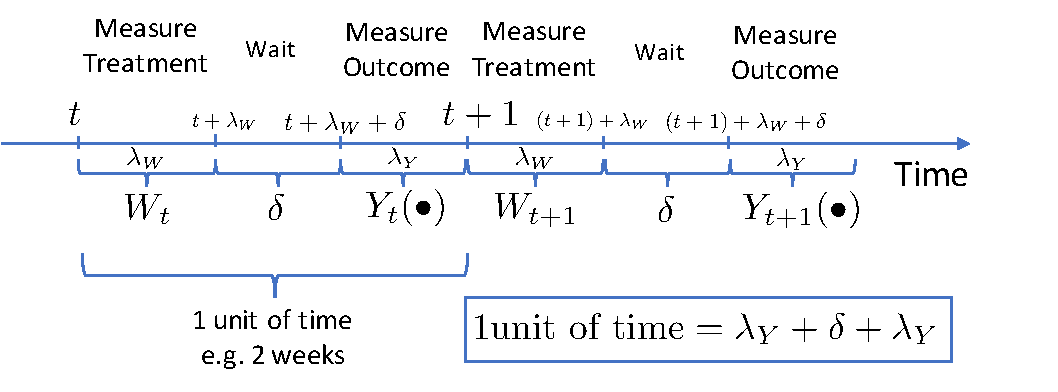
\includegraphics[width=0.75\textwidth]{time_figure_long_v3}
	\caption{Visualization of how the treatment and outcomes are defined over time. For example, $\lambda_W$ could equal 1 week and $\delta$ could equal a 1 week and $\lambda_Y$ could equal 2 weeks, then one unit of $t$ is equal to four weeks.}
	\label{fig:time_def}
\end{figure}

The potential outcomes at time 1 is then a function of whether or not unit $i$ contributed and some function of the total contributions of neighborhood of unit $i$,
\[
	Y_{i,1} (W_{i,1}, f(W_{\mathcal{N}_{i},1})),
\]
where $t$ subscript for the neighborhood has been suppressed in order to make the notation neater. Also, assume that 
$f(W_{\mathcal{N}_{i},1:t}) \in \mathcal{D}$, and we will denote generic values of $f(W_{\mathcal{N}_{i},1:t})$ as $D$ and specific realizations as lower case $d$. 
\begin{remark}
	The function $f(.)$ could take many different forms, such as a simple count, a mean or a weighted mean where the weights are derived from the influence a connection carries. I think PYMK team has been working on this idea. 
\end{remark}
Then, for any time $t$, the potential outcomes measure at $[t+\lambda_W +\delta, t+\lambda_W + \delta + \lambda_Y$ will be,
\[
	Y_{i,t} (W_{i,1:t}, f(W_{\mathcal{N}_{i},1:t})).
\]
If $\lambda$ is large enough (ideas how to check this are given below) then it will be reasonable to assume that the potential outcome is Markovian, in the sense that
\begin{align*}
	Y_{i,t} ((W_{i,1:t-1}, W_t), (f(W_{\mathcal{N}_{i},1:t-1}), f(W_{\mathcal{N}_{i},t}))) &= 
	Y_{i,t} ((W_{i,1:t-1}', W_t), (f(W_{\mathcal{N}_{i},1:t-1}'), f(W_{\mathcal{N}_{i},t}))) \\
	&= Y_{i,t} (W_t, f(W_{\mathcal{N}_{i},t})). 
\end{align*}

In words, the above equations say that the contributions at any time prior to $t-\lambda$ do not affect the outcome at time $t$. If this is true, then we have multiple observations from the same unit, which means that we should be able to get more accurate estimates of main and peer causal effect. 


\begin{remark}
	Simple check for Markov property of the potential outcomes: Fix a time point (we can run this for multiple time points) and compare all units that had $(W_{i,t-1}, W_{i,t}) = (0,1)$ and $(W_{i,t-1}, W_{i,t}) = (1,1)$; similarly compare all units that had $(W_{i,t-1}, W_{i,t}) = (1,0)$ and $(W_{i,t-1}, W_{i,t}) = (0,0)$. 
\end{remark}

\begin{remark}
	If the Markov assumption doesn't hold we can increase the value of $\lambda$ to increase the plausibility of this assumption.
\end{remark}


\subsection{Causal estimands} % (fold)
\label{sub:causal_estimands}
There are many different potentially interesting causal estimands. For now we focus on the following.

Main Effect:
\[
	\tau^M_{i,t}(1,0) = E[Y_{i, t+ \delta} (1,D) - Y_{i, t+ \delta} (0, D)].
\]
The main effect is ``averaging'' of the peer influence. In essence, we are going to end up treating the neighbors' contributions as a covariate and balance on it. Once we have balanced it, then the main effect can be estimated. This main effect (once averaged over all units) will be the average effect over the peer contributions. If desired, we can further analyze this effect for specific value of $d$ as it's possible for the main effect to change as a function of $d$. 

Peer Effect:
\[
	\tau^P_{i,t}(d,d') = E[Y_{i, t+ \delta} (m, d) - Y_{i, t+ \delta} (m, d')].
\]
Similar to the main effect we treat whether or not unit $i$ contributed as an important covariate. Here, it maybe of interest to consider how this peer effect changes for different value of $m$ and $m'$. 

Each of these effects can be average over time, to obtain the unit level average effect:
\[
	\tau^M_{i, \delta}(0,1) = \frac{1}{T} \sum_{t=1}^T \tau^M_i(1,0) \quad \tau^P_{i, \delta}(d,d') =  \frac{1}{T} \sum_{t=1}^T 
	\tau^P_{i,t}(d,d').
\]
Alternatively, we could average the causal effects across units. 

% subsection causal_estimands (end)
\section{Inference} % (fold)
\label{sec:inference}
In this section we discuss some strategies for attempting to estimate the causal effect. The effect we are trying to measure will dictate the method that we will use. 
% section inference (end)

\subsection{Inference for the main effect}

Estimation in this setting can be carried out using a propensity score (ps) matching method or inverse ps weighting. 
Treat whether or not user $i$'s ego contributed as an important covariate and bundle into the $X_{i,t}$.
Define the ps as
\[
  p_{i,t} = \Pr(W_{i,t} = 1 | X_{i,1:t}, W_{i,1:t-1}, Y_{i:t-1}^\text{obs}).
\]
\emph{Question}: Should we fit a different model for each unit, or should we fit a different one for time? I think the different one for each unit makes sense when we are analyzing the main effect. 


We can use the following estimator,
\[
	\hat \tau_{i,} = \frac{1}{T} \sum_{t=1}^T \frac{Y_{i,t }(1,-) W_{i,t}}{\hat p_{i,t}} - 
	\frac{Y_{i,t }(0,-) (1 - W_{i,t})}{1 - \hat p_{i,t}}.
\]
These should be unbiased as long as the propensity model is correct. We could also consider doing some level of smoothing to remove the sensitivity to the ps model. Also, at this point we could use a regression on the outcomes to do the ``doubly'' robust approach. 

Another approach is run a weighted regression of 
\[
	Y^\text{obs}_{it} = \alpha + \beta_t + \eta_{i} + \tau W_{it} + \zeta X_{i}
\]
then, $\tau$ will be an estimate of the average of the causal effects over the members and time, using the standardized weights,
\[
	\tilde p_{i,t} = \frac{\Pr(W_{i,t} = 1 | W_{i,1:t-1})} { p_{i,t}}.
\]
The important part of this regression is that there is a fixed effect for the time and member. This allows for any member variation to be account for, even if we do not have direct measurements of this variation.

\emph{Remark:} The above is assume that the potential outcomes are only a function of the current treatment assignment, however the treatment assignment is a function of the whole history of previous outcomes, treatment assignments and covariates. In practice, we of course assume that that is also only a function of say the last $t_k$ time steps. 

\subsection{Inference for the peer effect} % (fold)
\label{sub:inference_for_the_peer_effect}

We can attempt to use a similar approach, except the propensity score will now come from a Poisson distribution rather than a logistic as it will model the dose received. 

Alternatively, define only two kinds of units - these with highly active networks and these without. Then we can apply almost the same methodology to estimate the causal effect. 

% subsection inference_for_the_peer_effect (end)

\subsection{Extension to subclassification} % (fold)
\label{sub:extension_to_subclassification}

Subclassification is a must more stable approach to causal inference from observational studies, relative to IPW approaches. To apply in this setting we would at each time point $t$ we would use a subclassification algorithm to figure out appropriate groupings of the units. Then, we would use the weights (which are now counts) as the weights to use inside the final regression. Hopefully, this approach should be more stable. 
% subsection extension_to_subclassification (end)

\section{Diagnostic}

After analyzing an observational study, we need to perform checks and attempt to diagnose any failures. As standard practice we must check the balance that as achieved in the design stage of the observational study. On top of that, we could attempt to check the backwards causality assumption. Essentially we want to check if balancing indeed insured that the treatment assignment is independent of the outcome. To do this, we can run the following weighted regression:
\[
	W_{it} = \alpha + \tau' Y_{it}^\text{obs} + \beta_t' + \eta_{i}' + \zeta' X_{i}.
\]
If the balancing stage worked, then the estimate of $\tau'$ should be close to zero. 









































% \bibliographystyle{alpha}
% \bibliography{sample}

\end{document}